\cleardoublepage
\chapter{Koopmans functionals for periodic systems\label{ch:koopmans-periodic}}
In the previous chapter we described the general framework of Koopmans functionals, without focusing on the specific issues that arise when passing from finite to extended systems. Here, we address the issues that are particularly relevant when dealing with infinitely periodic systems, where the need for a localized set of orbitals brings about the apparent breaking of the translation symmetries of the system. The chapter is organized as follows: in Sec.~\ref{sec:localization}, we bring up the importance of having localized sets of variational orbitals in Koopmans functionals and Wannier functions are introduced; in Sec.~\ref{sec:bloch-theorem}, we discuss the validity of Bloch's theorem in the framework of ODD functionals, which represents one of the main results of this thesis; finally, Sec.~\ref{sec:koopmans-pbc} is devoted to the formulation of Koopmans functionals in periodic boundary conditions. As usual, we close with a small section that summarizes the content of the chapter.

Part of the content of this chapter has been published in Refs.~\cite{de_gennaro_blochs_2022} and \cite{colonna_koopmans_2022}.

\clearpage
\section{The importance of localization\label{sec:localization}}
Two important aspects underlie the forthcoming discussion about the localization in Koopmans functionals: (i) the discussion at the end of Sec.~\ref{sec:deriv-dis}, and (ii) the nature of the KI correction [see Eq.~\eqref{eq:ki-correction}]. The effects of the orbitals localization on the derivative discontinuity and on the PWL were already touched upon, whereas the impact that such effects can have in infinitely periodic systems, and how this affects Koopmans corrections is the topic of this section.

As usual, we start from standard DFT. It is known that local and semi-local DFAs tend to spread the orbitals as much as possible over the whole system's extension. This is a consequence of the self-interaction error or, equivalently, the deviation from the PWL that affects such approximations, to the point that it has been suggested by Mori-S\'{a}nchez \emph{et al.} to interpret the failures of local functionals in terms of a \emph{delocalization error} \cite{mori-sanchez_localization_2008}. The orbitals delocalization modifies the way the energy deviates from the exact PWL behavior\footnote{Once more, we remark that a correct PWL consists of two equally important features: (i) the linear trend at fractional occupations, and (ii) the correct estimation of the energies on either side of each linear segment, namely the energies at integer numbers of electrons. The fulfillment of the first requirement only, brings to a curve which is, indeed, piecewise-linear, but without the correct slope of the linear segments; in this sense, we consider such a curve to be deviating from the (exact) PWL behavior.}: for finite systems -- the limited extension of the system does not let the orbitals to delocalize too much -- the energy profile is the one showed in the red curve of Fig.~\ref{fig:deviation-pwl}, where the energies at integer points are quite correct, while at fractional occupations we observe a mistaken non-linear convex trend; by increasing the size of the system, the orbitals delocalization increases and the non-linear trend progressively turns into a linear one, while the relative position of the energies at integer numbers of electrons decreases. Such behavior is a natural consequence of the convexity of approximated energy functionals: if we consider a periodic system made of $M$ repetitions of the unit cell, each of which contains $N$ electrons, and we imagine to add a fraction $\delta$ of an electron, Eq.~\eqref{eq:convexity} shows that local functionals will split the electron -- equally, in order to preserve the translation symmetry of the system -- among the different unit cells. The total ground-state energy of the system then reads as \cite{mori-sanchez_localization_2008}
%
\begin{equation}
    \begin{split}
    E^{\rm DFA}(NM + \delta) &= M E^{\rm DFA}\left( N + \frac{\delta}{M} \right) \\
    &= ME^{\rm DFA}(N) + \delta \left. \frac{dE^{\rm DFA}}{dN} \right|_{N+\delta} + \mathcal{O} \left( \frac{\delta^2}{M} \right) .
    \end{split}
    \label{eq:pwl-convex-to-linear}
\end{equation}
%
When approaching the thermodynamic limit ($M\longrightarrow \infty$), the dependence of the energy on $\delta$ becomes more and more linear; moreover, thanks to Janak's theorem
\footnote{The \emph{aufbau} principle tells us that the change in the ground-state energy due to a variation in the number of particles, is equivalent to the one coming from a variation in the occupation of the HO orbital; the Janak's theorem for the HO orbital can then be rewritten as a derivative with respect to the total number of particles:
\begin{equation*}
    \frac{dE}{dN} = \frac{dE}{df_{\rm HO}} = \varepsilon_{\rm HO} .
\end{equation*}
}, 
Eq.~\eqref{eq:pwl-convex-to-linear} shows that the derivative of the energy equals the KS highest-occupied eigenvalue, which strongly underestimates the IP of the system. To summarize, when dealing with infinitely extended systems, the energy of local and semi-local density-functionals shows a linear trend that, at a first sight, might resemble the exact PWL behavior; however, it turns out that, differently from what happens in small finite systems where the orbitals remain localized and $\Delta$SCF-like calculations provide an accurate prediction of ionization energies, here the separation between energies at integer points is strongly underestimated, meaning that not only energy derivatives, but also total energy differences (where an electron was removed from, or added to, a delocalized KS orbital), miss completely the ionization energies of the system.

\begin{figure}
    \centering
    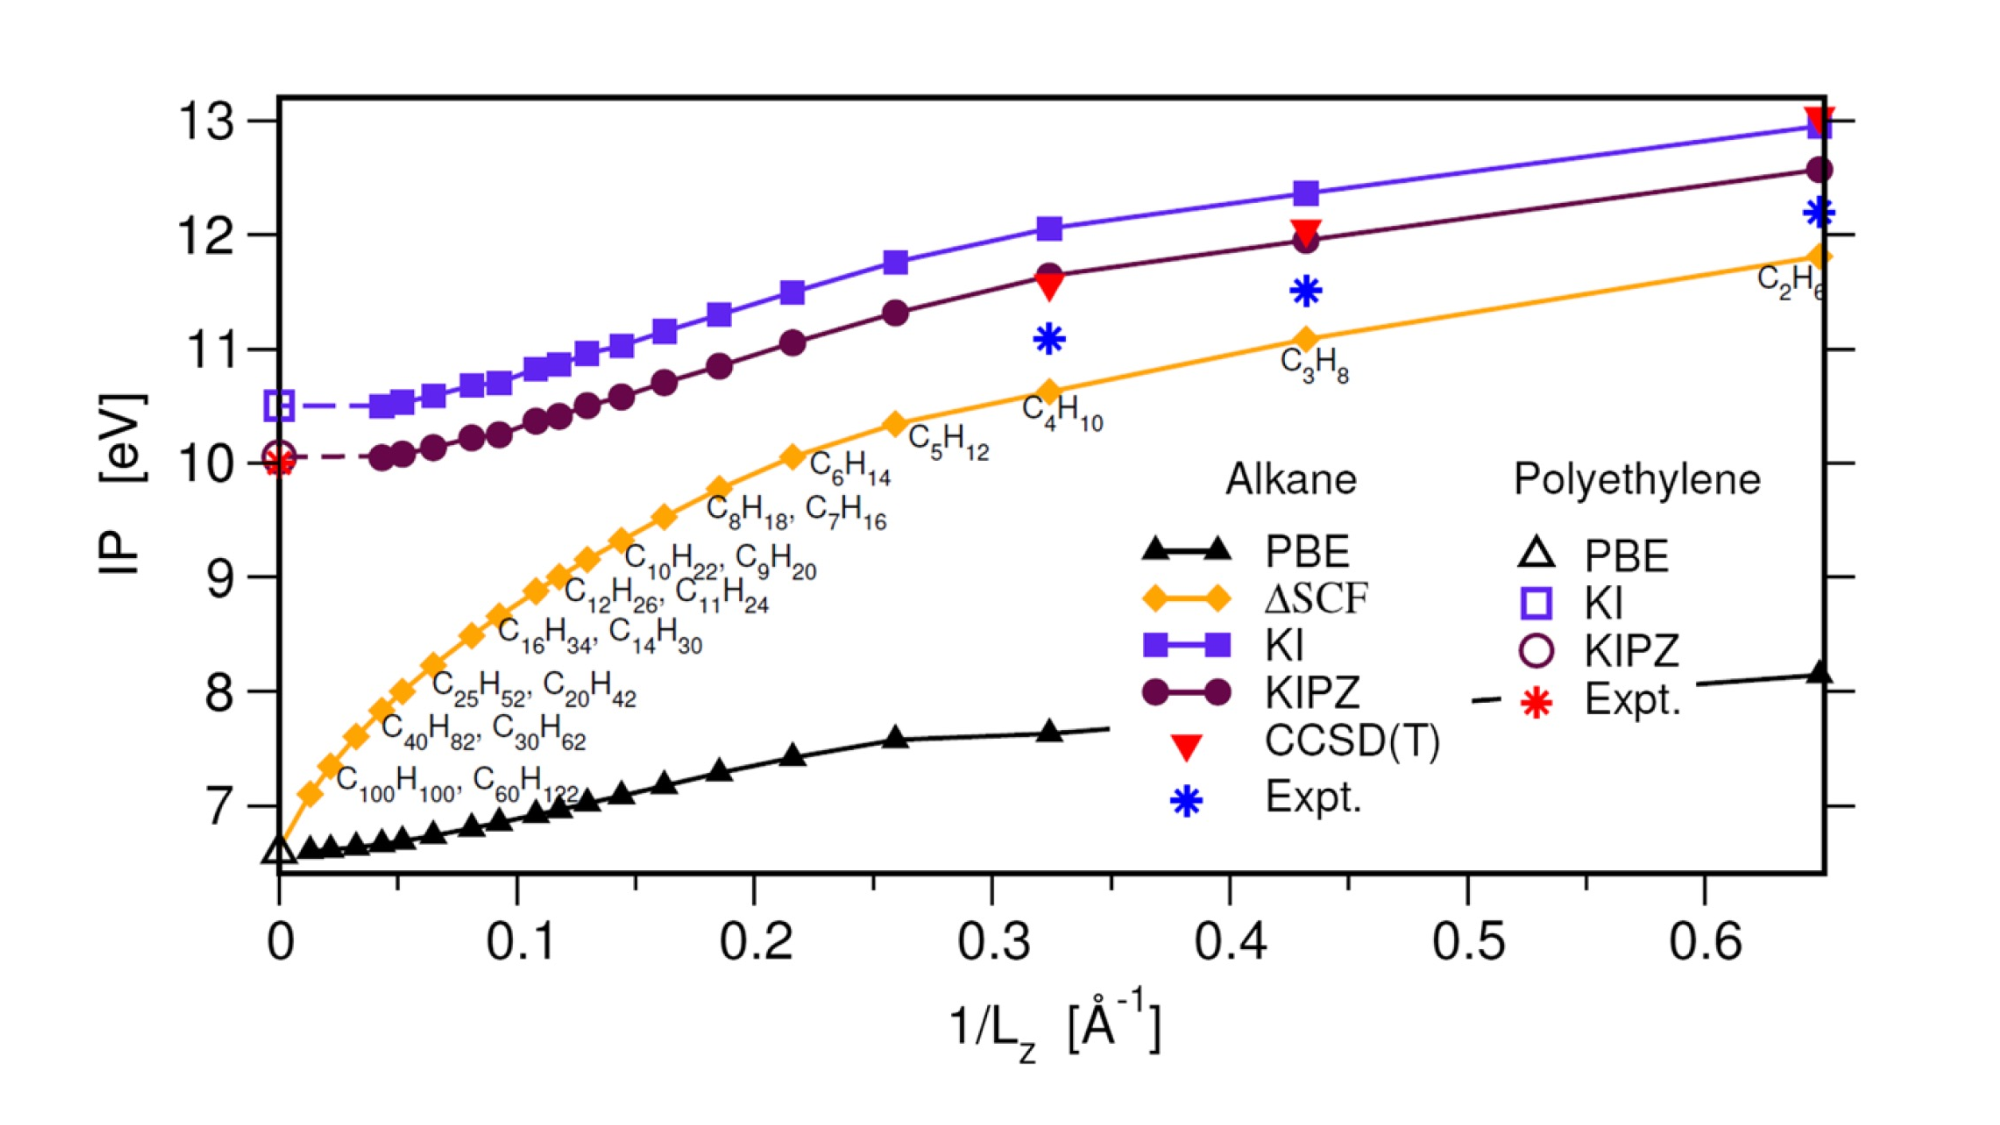
\includegraphics[width=0.85\linewidth]{IP-alkane-chain.pdf}
    \caption[PBE, KI, and KIPZ IPs for the alkane chain.]{A study taken from Ref.~\cite{nguyen_koopmans-compliant_2018}, where the authors compared the performance of PBE, KI, and KIPZ for the calculation of the IP of the alkane chain, $C_n H_{2n}$, at different lenghts, and of polyethylene (infinite limit). The KI and KIPZ IPs are taken as the negative of the HO eigenvalue, while for PBE both $\varepsilon_{\rm HO}$ and the $\Delta$SCF value were considered. At the PBE level, while the opposite of $\varepsilon_{\rm HO}$ strongly underestimates the IP at any lenghts, the $\Delta$SCF value provides accurate predictions at small lenghts and, because of the orbital delocalization, it gets progressively worse when the size of the system increases. We remark that, at the thermodynamic limit, the $\Delta$SCF value recovers the negative of the KS HO eigenvalue. On the other hand, both the Koopmans flavors perfectly agree with coupled-cluster and experimental results (red triangles and star), even at the infinite limit, where the orbitals are represented by Wannier functions.}
    \label{fig:ip-alkane-chain}
\end{figure}

The failure of local and semi-local DFAs to describe delocalized states becomes crucial when Koopmans corrections are introduced. As we mentioned repeatedly, the KI correction linearizes the energy of the base functional at fractional occupations, and it retains it at integer points. Therefore, for a functional that is already linear, the $\Pi_i^{\rm KI}$ terms of Eq.~\eqref{eq:pi-term-general}, or Eq.~\eqref{eq:ki-correction}, are identically zero. In order to have effective Koopmans corrections in extended systems, it is necessary to switch to a localized representation of the electronic states, where the energy does not vary linearly with respect to a change in the orbital occupations. Rather than considering the Bloch-like KS states, Koopmans functionals resort to sets of localized orbitals -- e.g., Wannier functions -- where the constrained $\Delta$SCF energy differences related to variations in the filling of such orbitals yield, presumably, good results (as shown in Fig.~\ref{fig:ip-alkane-chain}).

The advantage of using localized orbitals has driven many DFT-based methods that aimed to describe excited-state properties of periodic systems -- some of those introduce corrections that closely resemble the KI functional. To mention a few we find: the transition-state method proposed by Anisimov and collaborators, which generalizes Slater's $1/2$-method by improving the definition of the ionization energies -- rather than taking the values of the energy curvature, $\partial \varepsilon_i / \partial f_i$, at half occupation, these are computed self-consistently via constrained DFT calculations -- and by replacing the KS Bloch states, for which the applied corrections vanish in extended systems, with Wannier functions \cite{anisimov_transition_2005,anisimov_orbital_2007}; the range-separated dielectric-dependent hybrid functionals developed by Wing \emph{et al.}, where the optimal value of the range-separation parameter is determined by imposing the Koopmans condition on the Wannier functions, rather than on the delocalized KS states \cite{wing_band_2021}; the Wannier-Koopmans method developed in the group of L.-W. Wang, which augments the LDA Hamiltonian with Wannier-based $\Delta$SCF-like terms \cite{ma_using_2016,ma_energy_2016,weng_wannier_2017,weng_wannier_2018,li_wannier-koopmans_2018,weng_wannierkoopmans_2020}; similar corrections are used also in the localized orbital scaling correction (LOSC) scheme developed by W. Yang and collaborators, who make use of Wannier-like \emph{orbitalets} (orbitals obtained by finding the optimal compromise between the localization in space and in energy) \cite{li_localized_2018,mei_libsc_2021,mahler_wannier_2022}.

Also in PZ-SIC functionals, the orbitals localization plays a fundamental role: the density of a delocalized orbital is locally very small, and the correspondent self-Hxc energy tends rapidly to zero. This explains why PZ corrections vanish in the limit of infinitely extended systems, and provides further evidence for the disappearance of Koopmans corrections:
%
\begin{equation}
    \begin{split}
    \Pi_i^{\rm uKI} &= E^{\rm DFT}[\rho - \rho_i] - E^{\rm DFT}[\rho] + f_i \left( E^{\rm DFT}[\rho - \rho_i + n_i] - E^{\rm DFT}[\rho - \rho_i] \right) \\
    &\approx E^{\rm DFT}[\rho] - E^{\rm DFT}[\rho] + f_i \left( E^{\rm DFT}[\rho] - E^{\rm DFT}[\rho] \right) = 0 .
    \end{split}
    \label{eq:vanishing-ki-correction}
\end{equation}
%
The minimization of the PZ energy naturally brings to a set of localized orbitals\footnote{We point out that, in order to localize the orbitals, SIC schemes often require the initial guess to be already localized, whereas starting from delocalized orbitals might bring to local minima where the orbitals are still delocalized \cite{korzdorfer_relation_2011}.}, for which the magnitude of $E_{\rm Hxc}[\rho_i]$ increases and the system reaches a more energetically favorable configuration (the self-Hxc are preceded by the negative sign, thus the energy is minimized by maximizing such terms). In this sense, the Pederson condition, which provides the energy minima within a particular subspace, is also interpreted as a \emph{localization condition}. Given the close connection between Koopmans and PZ functional gradients -- we remind that KIPZ is the KI correction applied to a screened PZ functional, while KI can be seen as a KIPZ functional with a vanishigly small PZ term -- the minimization of Koopmans functionals benefits from the same ``natural'' predisposition to localize orbitals. Ultimately, this allows to have effective Koopmans corrections also in the limit of extended systems, as demonwhich brings to effective corrections also in extended systems. 

\subsection{Wannier functions\label{sec:wannier-functions}}
When dealing with periodic systems, the most natural choice for a set of localized orbitals is represented by Wannier functions (WFs). The reason is that WFs possess important properties that carry all the information about the translation symmetries of the system. Moreover, WFs are strictly connected to Bloch functions, as they reciprocally play the role of Fourier transforms of the other, which makes them the dual representation of Bloch states.

In order to draw the attention to the translation properties of WFs, we first consider a simplified definition (for single-band systems), and refer to the second part of this section for the most general definition. Given the set $\{ \psik \}$ of Bloch functions, where $\bk$ are the crystal vectors living within the first Brillouin zone (BZ) of the system, the Wannier function $\wR$ corresponding to the Bravais lattice vector $\bR$ is defined as
%



\section{Bloch's theorem in ODD functionals\label{sec:bloch-theorem}}

\subsection{Bloch's theorem\label{sec:bloch-theorem-sub}}

\subsection{Validity in standard DFT\label{bloch-th-dft}}

\subsection{Validity in ODD functionals\label{sec:bloch-th-odd}}

\section{Koopmans functionals in periodic boundary conditions\label{sec:koopmans-pbc}}

\section{Summary\label{sec:ch4-summary}}

